% Chapter Template

\chapter{\studio} % Main chapter title

\label{Chapter3} % Change X to a consecutive number; for referencing this chapter elsewhere, use \ref{ChapterX}

\lhead{Cap\'itulo 3. \emph{\studio}} % Change X to a consecutive number; this is for the header on each page - perhaps a shortened title

%----------------------------------------------------------------------------------------
%	SECTION 1
%----------------------------------------------------------------------------------------

\section{La Aplicación \studio}
\studio consiste en una aplicación distribuida con un cliente web y un cliente Android respaldados ambos por un servidor construido sobre el framework web para Python, Django.\\
Esta aplicación se construye ante la necesidad de poder visualizar la escena actual durante el desarrollo. El proceso natural del desarrollo en Android consiste en inclusión de recursos, construcción del proyecto e instalación en el dispositivo. Realizar esta costosa operación para pequeños cambios como podría ser una pequeña traslación de un objeto, rotar la cámara,... llega a ser un proceso lento y tedioso, gracias a \studio se consigue visualizar el estado de la escena de forma instantánea.

\section{Blender Scripting}
Como se ha dicho, el motivo de existir de \studio se basa en la necesidad de simplificar el desarrollo, y entre esas tareas está el poder ofrecer un entorno completo en el que, hasta la exportación de las escenas almacenadas en blender se simplifique.\\

Para la exportación desde Blender se hace uso de la API para Python.\\
Se explicará a continuación la estructura que sigue el script de exportación.\\

\subsection{Datos}
Los datos obtenidos de Blender, como podrían ser los vértices de las mallas, la localización de los huesos,... se almacenan en objetos planos.\\
Haciendo uso de la biblioteca de JSON para Python convertiremos estos objetos en instancias JSON una vez haya finalizado el proceso de exportación.

\subsection{Exportadores}
Los exportadores son los elementos fundamentales encargados de convertir objetos de Blender a los objetos planos que serán exportados.\\
Cabe destacar que mientras que algunos exportadores son relativamente sencillos como podrían ser los exportadores de los materiales otros 

TODO: Explicar como funciona el script de blender y como se exportan algunas secciones importantes como una Mesh, las animaciones,...

\section{La Aplicación Django}

\begin{figure}[h!]
\begin{center}
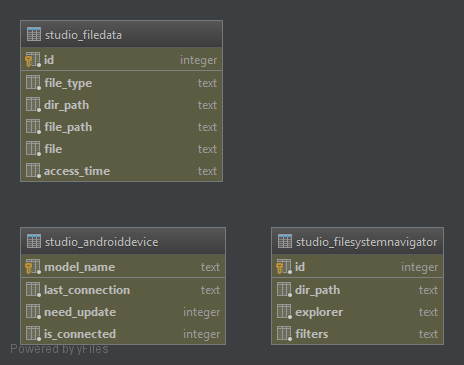
\includegraphics[scale=0.7]{djangodiagram.png}
\end{center}
\caption[Datos almacenados en \studio]{Datos almacenados en \studio}
\end{figure}

TODO: Explicar la aplicación servidor, la pequeña base de datos SQLite usada, servicios implementados

\section{Cliente Web}
TODO: Comentar las distintas páginas y acciones a realizar en cada una

\section{Cliente Android}
El ciente Android es la parte de la aplicación que hace de mensajero entre el servidor Django y \robotto.\\
Está construída como una aplicación sencilla y ligera para evitar 

TODO: Comentar como utilizar cada acción, como hace para actualizarse de forma automática, servicios a los que se conecta